\chapter{Separating multilinear ABPs and formulas}\label{chap:DMPY}

So far we have seen that the partial derivative matrix can be used to exhibit a weakness of multilinear formulas. Furthermore, this also yielded a separation between circuits and ABPs as we also saw a construction of a \emph{full-rank}  polynomial by a linear sized multilinear circuit.

A natural question now is where multilinear ABPs sit? We do know that multilinear ABPs are sandwiched between multilinear formulas and multilinear circuits and hence one of the two containments has to be strict.

\begin{definition}[Multilinear ABPs]

\end{definition}

Dvir, Malod, Perifel and Yehudayoff~\cite{dmpy12} proved that multilinear formulas are strictly contained multilinear ABPs. Formally, they prove the following result.

\begin{theorem}[\cite{dmpy12}]
\label{thm:separation}
For every $m \in \mathbb{N}$, there is an explicit polynomial $F_n$ on $n = \poly(m)$ variables $\vecx = \inbrace{x_1,\ldots,x_n}$ such that
\begin{itemize}
\item $F$ is computable by a multilinear algebraic branching program of size $O(n^2)$,
\item any multilinear formula computing $F$ requires size $n^{\Omega(\log n)}$.
\end{itemize}
\end{theorem}

It is worth noting that one can not get an asymptotically better separation than this, as any $\poly(n)$ sized multilinear circuit can be converted into a multilinear formula of size $n^{O(\log n)}$.
Therefore, among other things this result tells us that a better reduction from circuits to formulae is not possible at least in the multilinear regime.

\subsection*{Proof idea}

The outline of the proof follows that of Raz's proof \cite{raz2004} of a quasipolynomial lower bound for the \emph{full-rank-polynomial} against multilinear formulae that we saw in \autoref{chap:multilinear}. That is it used the \emph{log-product decomposition} for multilinear formulae, and showed that the decomposition is ``rank deficient'' under a uniformly random equipatition of the variable set, with high probability.

At this point, a possible line of argument is to use Raz's full-rank-polynomial and show that it is computable by multilinear ABPs. However, it is not known that it is possible. The idea of Dvir et. al. is to construct a different polynomial that is full-rank for a certain \emph{subset of restricted partitions}, and choose this subset of partitions carefully so that the polynomial is computable by ABPs. 
This carefully chosen set of partitions is referred to as \emph{arc partitions} in the proof. The name becomes fairly clear from the process of ``sampling'' an arc partition, which is what has been used to describe the distribution.

The harder part is to show that Raz's lower bound proof continues to hold even for just these restricted partitions. That is, we now need to show that the log-product decomposition is rank deficient under a random \emph{arc partition} with high probability. This proves to be quite tricky and a large chunk of the proof is just that, as we will soon see in the rest of this chapter. 

\section{Arc partitions}

As mentioned above, the full-rank-polynomial as used in \cite{raz2004} need not be computable by multilinear ABPs. We will therefore have to work with a polynomial that has full rank under a smaller set of partitions. We will call these partitions as \emph{arc partitions}, which will be characterised by the support of the distribution $\mathcal{D}$ of the random process given below.

The random process will first pick $n/2$ pairs from $\vecx$ and then ``bicolour'' each pair with $\vecy$ and $\vecz$ uniformly at random, to obtain an equipartition. Imagine the indices of $\vecx$ from $[n]$ arranged in order on an $n$-cycle, in a clockwise manner. The following example of such a partition from this distribution should help understand the formal sampling process. 

\vspace{0.5em}

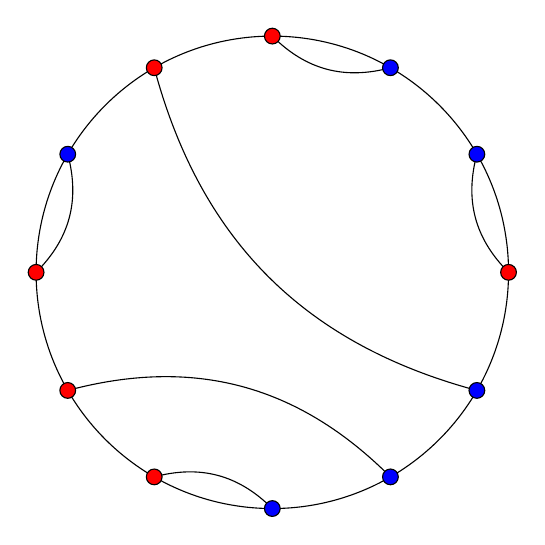
\begin{tikzpicture}
  \draw[draw] (0,0) circle (3cm);
  \draw[thin,black] (90:3) to[bend right]  (60:3);
  \draw[thin,black] (30:3) to[bend right] (0:3);
  \draw[thin,black] (120:3) to[bend right] (-30:3);
  \draw[thin,black] (180:3) to[bend right] (150:3);
  \draw[thin,black] (210:3) to[bend left] (300:3);
  \draw[thin,black] (240:3) to[bend left] (270:3);

  \draw[fill=red] (0:3) circle (0.1cm);
  \draw[fill=blue] (30:3) circle (0.1cm);
  \draw[fill=blue] (60:3) circle (0.1cm);
  \draw[fill=red] (90:3) circle (0.1cm);
  \draw[fill=red] (120:3) circle (0.1cm);
  \draw[fill=blue] (150:3) circle (0.1cm);
  \draw[fill=red] (180:3) circle (0.1cm);
  \draw[fill=red] (210:3) circle (0.1cm);
  \draw[fill=red] (240:3) circle (0.1cm);
  \draw[fill=blue] (270:3) circle (0.1cm);
  \draw[fill=blue] (300:3) circle (0.1cm);
  \draw[fill=blue] (330:3) circle (0.1cm);
\end{tikzpicture}

\vspace{0.5em}

The random process begins with the singleton set of pairs $P_1 = \inbrace{\inbrace{0,1}}$. The process then picks one pair of unpicked elements in each iteration, till there are no more elements to pick. Throughout the process of picking these $n/2$ pairs, it maintains the invariant that all the pairs picked till some iteration $t$, together cover exactly a contiguous arc of length $2t$ on the cycle. Let the set of pairs picked ater iteration $t$ be $P_t$, and let the corresponding arc be $\insquare{L_t, R_t}$, with $R_t - L_t \equiv 2t (\bmod n)$. Under the given restrictions there are three choices for the next arc to be picked, and the process picks one of these uniformly at random. That is:
\[
	P_{t+1} =
	\begin{cases}
		P_t \cup \inbrace{\inbrace{L_t - 2, L_t - 1}} &\text{w.p. } \frac{1}{3}\\ 
		P_t \cup \inbrace{\inbrace{L_t - 1, R_t + 1}} &\text{w.p. } \frac{1}{3}\\
		P_t \cup \inbrace{\inbrace{R_t + 1, R_t + 2}} &\text{w.p. } \frac{1}{3}\\
	\end{cases}
\]
Here the additions and subtractions on the indices are \emph{modulo} $n$. Let the final set of $n/2$ pairs be $P = P_{\frac{n}{2}}$. The process now goes over all pairs inside $P$ and colours one variable by $\vecy$ and other by $\vecz$, uniformly at random to obtain the equipartition.

For ease of notation, we will say that both the set of $n/2$ pairs $P$ and the actual partition $\pi(P)=\vecy \sqcup \vecz$ are generated using $\mathcal{D}$. That is, we will use both $\pi(P) \sim \mathcal{D}$ and $P \sim \mathcal{D}$. As we mentioned earlier, the set of arc partitions is exactly the support of this distribution $\mathcal{D}$. Similarly, an \emph{arc-full-rank} polynomial will be a polynomial $f$ for which $M_{\vecy,\vecz}(f)$ has rank $2^{n/2}$ for every arc partition $\vecy,\vecz$.\\

The task is now in two parts. The first is to show that we can find a multilinear ABP that computes an \emph{arc-full-rank} polynomial $f$. Then, we have to show that any small multilinear formula is rank-deficient under a random arc-partition. 

\section{Upper bound with ABPs}

We want the hard polynomial to have full rank with respect to every arc partition, so let us see how we can come up with a full rank polynomial for a fixed partition $\vecy \sqcup \vecz$. Say $\vecy = \inbrace{y_1,\ldots,y_m}$ and $\vecz = \inbrace{z_1,\ldots,z_m}$. We know that the polynomial $P(\vecy,\vecz) = \Pi_{i \in [m]} (y_i + z_i)$ has full rank with respect to the given partition.

Now we want to extend this idea to having full rank over any arc partition. One way to do this is to add a few (at most polynomially many) extra variables $\vecw$ so that for any arc partition $\pi$ there will be an assignment $\phi$ to $\vecw$ that will ensure that $F_n(\phi(\vecw),\pi(\vecx))$ looks like $P(\vecy,\vecz)$. We are going to do just that and additionally ensure that $F_n$ is still computable by a small multilinear ABP.

Recall that for sampling of pairs from $\mathcal{D}$ we maintained the invariant that the pairs in $P_t$ cover a contiguous arc $\insquare{L_t, R_t}$ of length exactly $2t$ on the $n$-cycle. This gives us that for any $t$, after $t$ steps the number of distinct $P_t$s possible, is at most $n$. Moreover for the $(t+1)^{th}$ sampling step it is enough just to know $L_t$ and $R_t$. This helps us construct the following ABP of width $\leq n$ and $n/2$ layers, that we describe by describing the underlying graph.\\

Let the nodes in each layer $t$ be labelled as $v_1^{(t)},\cdots, v_n^{(t)}$. The node $v_i^{(t)}$ would correspond to the fact that the current arc is $[i,i+2t] \bmod{n}$. The edges of the ABP are as follows. There would be three edges out of $v_i^{(t)}$ and they are as follows:

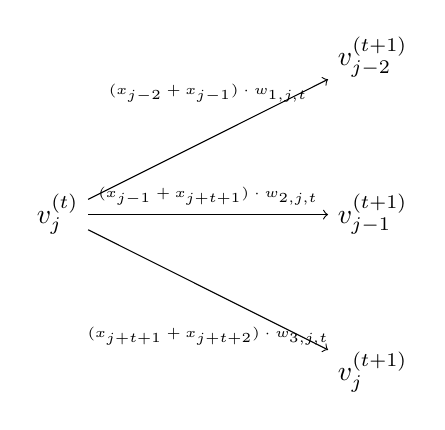
\begin{tikzpicture}
  \node (vj) at (0,0) {$v_j^{(t)}$};
  \node (v1) at (4,2) {$v_{j-2}^{(t+1)}$}
  edge[<-] node [midway,above=10pt] {{\tiny $(x_{j-2} + x_{j-1})\cdot w_{1,j,t}$}} (vj);
  \node (v2) at (4,0) {$v_{j-1}^{(t+1)}$}
  edge[<-] node [midway,above] {{\tiny $(x_{j-1} + x_{j+t+1})\cdot w_{2,j,t}$}} (vj);

  \node (v3) at (4,-2) {$v_{j}^{(t+1)}$}
  edge[<-] node [midway,below=10pt] {{\tiny $(x_{j+t+1} + x_{j+t+2})\cdot w_{3,j,t}$}} (vj);
\end{tikzpicture}

The ABP therefore has $O(n^2)$ vertices and since there are three edges out of each vertex, there are $O(n^2)$ edges. The polynomial computed by the ABP, $F_n$, would be our hard polynomial. From the construction, the following lemma is easy to verify and is left as an easy exercise.

\begin{exercise}
  Show that the polynomial $F_n$ constructed above is full-rank with respect to every arc-partition.
\end{exercise}


\subsection{Lower bound against formulae}

As discussed earlier, we will prove the lower bound by proving that the probability of a \emph{log-product term} having rank that is $n^{\delta}$ close to full is inverse quasipolynomially small. Then for any polynomial sized formula, we will simply use the union bound to show that is cannot compute the polynomial $F_n$.

\begin{theorem}
\label{thm:logProdRankBound}
Let $g \in \F[\vecx]$ be a \emph{log-product term} and $\mathcal{D}$ be the arc partition distribution. Then there exists a constant $\delta$ such that
\[
\qquad \qquad \qquad \qquad \Pr_{\pi(P)=\vecy,\vecz \sim \mathcal{D}} \insquare{\operatorname{rank}\inparen{M_{Y,Z}(g)} \geq 2^{n/2 - n^{\delta}}} \leq n^{-\Omega(\log n)}.
\]
\end{theorem}

We will first see why we are done if we have the above theorem. By \autoref{obs:partialProps} combined with \autoref{lem:logProductFormula} and the union bound, if we have a formula of size $s$ that computes the \emph{arc-full-rank} polynomial $F$, then we can say the following.
\begin{align*}
1 &\leq \Pr_{\vecy,\vecz \sim \mathcal{D}} \insquare{ \operatorname{rank}\inparen{M_{\vecy,\vecz}(F)} \geq 2^{n/2}}\\
  &\leq \Pr_{\vecy,\vecz \sim \mathcal{D}} \insquare{ \operatorname{rank}\inparen{M_{\vecy,\vecz}(F_1 + \cdots + F_{s+1})} \geq 2^{n/2}} \text{where each $F_i$ is a \emph{log-product} polynomial}\\
  &\leq \Pr_{\vecy,\vecz \sim \mathcal{D}} \insquare{ \sum_{i \in [s+1]} \operatorname{rank}\inparen{M_{\vecy,\vecz}(F_i)} \geq 2^{n/2}}\\
  &\leq (s+1) \Pr_{\vecy,\vecz \sim \mathcal{D}} \insquare{ \exists i : \operatorname{rank}\inparen{M_{\vecy,\vecz}(F_i)} \geq 2^{n/2}/(s+1)}\\
  &\leq (s+1) \Pr_{\vecy,\vecz \sim \mathcal{D}} \insquare{ \exists i : \operatorname{rank}\inparen{M_{\vecy,\vecz}(F_i)} \geq 2^{n/2 - n^{\delta}}}\\
  &\leq (s+1) n^{-\Omega(\log n)}.
\end{align*}
Therefore we get that $s = n^{\Omega(\log n)}$, which proves the lower bound in \autoref{thm:separation}. Let us now prove the result from \autoref{thm:logProdRankBound}.

We want to upper bound the probability of a log-product term having rank that is $n^{\delta}$-close to full. The product case from \autoref{obs:partialProps} tells us that this can be achieved by saying that many of the $\vecx_i$s are imbalanced beyond the $n^{\delta}$ threshold with high probability. Note that if $\vecx_i$ picks up lot of ``whole pairs'' from the set of pairs $P$ obtained from $\mathcal{D}$, then no colouring of those pairs can push $\vecx_i$ towards imbalance. It is therefore sensible to look at buckets that pick up exactly one element from a lot of pairs. For that purpose, we define the following quantities for a fixed set of pairs $P \sim \mathcal{D}$ and a partition $\vecx = \vecx_1 \sqcup \vecx_2 \sqcup \cdots \sqcup \vecx_K$ given by some log-product term, as defined above.
\[
	\qquad V_k(P) = \inbrace{ p \in P : \abs{ p \cap \vecx_k } = 1 }
	\qquad \qquad \qquad \qquad 
	G(P) = \inbrace{ k \in [K] : \abs{ V_k(P) } \geq n^{1/1000} }
\]

Now our intuition from above translates to saying that a sizeable fraction of the $K$ buckets will end up in $G(P)$. The following lemma which is the technical bulk of the paper states exactly that.

\begin{lemma}
\label{lem:manyBucketsWithCuts}
Given a partition $\vecx = \vecx_1 \sqcup \cdots \sqcup \vecx_K$ with $K = \Theta(\log n)$ and $\abs{\vecx_i} \geq n^{7/8}$ for all $i \in [K]$
\[
	\qquad \qquad \qquad \qquad \qquad \qquad \Pr_{P \in \mathcal{D}} \insquare{ \abs{G(P)} \leq K/1000 } \leq n^{- \Omega(K)}
\]
where $\mathcal{D}$ is the distribution for arc partitions.
\end{lemma}

We will see a sketch of the proof of the lemma in the next section. For now, let us assume the lemma and finish the proof of the main theorem. The lemma gives us $\Omega(\log n)$ buckets that cut a lot of pairs. Assume the buckets are $\vecx_1,\ldots,\vecx_{K'}$ without loss of generality. Suppose now we colour the pairs that $\vecx_1$ cuts at random. We will then get an inverse polynomial upper bound on the colouring of these pairs being $n^{\delta}$-close to balanced, for some small enough constant $\delta$. However if we now want to argue the same for $\vecx_2$, we need to ensure that a polynomial number of pairs that it cuts remain uncoloured even after the previous colouring. Note that if for every $\vecx_i$ we can ensure that even after the colouring of pairs cut by $\inbrace{\vecx_1,\ldots,\vecx_{i-1}}$, polynomially many pairs cut by $\vecx_i$ are left uncoloured, then we get a bound that looks like $\inparen{n^{-\Omega(1)}}^{K'}$. This will mean that given any bucketing, the total probability of the colouring being $n^{\delta}$-balanced will be upper bounded by $n^{-\Omega(\log n)}$. It is not clear that we can make such a statement about all the buckets in $G(P)$. However, we will now see that we can indeed make a similar statement by taking a hit of not more than a constant.

Define a graph $H(P)$ with the buckets $\inbrace{\vecx_1,\ldots,\vecx_K}$ as vertices and edges between $\vecx_k$ and $\vecx_{k'}$ if there exist more than $n^{1/1500}$ pairs that intersect with both $\vecx_{k}$ and $\vecx_{k'}$. Let $G(P) = \inbrace{\vecx_1,\ldots,\vecx_{K'}}$. Note that since each bucket from $G(P)$ cuts $\geq n^{1/1000}$ pairs and since there are at most $O(\log n)$ other buckets to share them with, every vertex from $G(P)$ has degree at least 1.

\begin{lemma}
\label{lem:halfVerticesIndep}
There exists a sequence $B=\inparen{b_1,\ldots,b_r}$ of vertices from $H(P)$, that are also in $G(P)$, of size $\geq K'/2 - 1$ such that for all $i \in [r]$, in the graph obtained from $H(P)$ by deleting $\inbrace{b_1,\ldots,b_{i}}$, each vertex from $\inbrace{b_{i+1},\ldots,b_{r}}$ has degree $\geq 1$.
\end{lemma}
\begin{proof}
We will prove this lemma by induction on the number of vertices from $G(P)$ present in the graph. If there are at most 2 vertices from $G(P)$, then the lemma is vacuously true. The base case with 3 vertices from $G(P)$ is easy to see. Therefore let us now prove the inductive step, assuming there are $\ell \geq 3$ vertices from $G(P)$ in the graph. In this graph, pick a vertex from $G(P)$ that has the minimum degree. Let it be $h_1$. Deleting $h_1$ can make at most one vertex from $G(P)$ isolated in the new graph. If such a vertex exists, call it $h'_1$. Now delete both $h_1$ and $h'_1$. We now have a graph that has at least $(\ell - 2)$ vertices from $G(P)$, with the guarantee that each of them has degree at least 1. We now apply the inductive hypothesis to obtain a sequence $(b'_1,\ldots,b'_{t})$ with $t \geq \ell/2 - 2$. We can therefore safely produce $(h_1,b'_1,\ldots,b'_{t})$ as the sequence for the graph we started with.
\end{proof}

Let $(b_1,\ldots,b_r)$ be such a sequence for $H(P)$, with $r \geq K'/2 - 1 = \Omega(K)$. For brevity, let pairs that are not cut by any of the $b_i$s be $\tilde{P}$. For every $i \in [r]$, define by $P_i$ the pairs from $\inparen{ P \setminus \inparen{ P_1 \cup \cdots \cup P_{i-1}} }$ that are cut by $b_i$. Now view the random colouring $\pi(P)$ of pairs from $P$ to be happening in the order $P_1,\ldots,P_r,\tilde{P}$. From \autoref{lem:halfVerticesIndep} we have that $\abs{P_i} \geq n^{1/1500}$ for all $i \in [r]$. As mentioned above, this will help us yield an inverse polynomial factor for each of the $r$ buckets, even after conditioning on previous colourings. Also let $n_i = \abs{b_i}$ and for $\pi(P)=\vecy,\vecz \sim \mathcal{D}$, let $y_i = \abs{b_i \cup \vecy}$. In the case when $\abs{G(P)} \geq K/1000$, we therefore get that
\begin{align*}
\Pr_{\pi(P)=\vecy,\vecz \sim \mathcal{D}} \insquare{\operatorname{rank}\inparen{M_{Y,Z}(g)} \geq 2^{n/2 - n^{\delta}}} &\leq \Pr_{\pi(P)=\vecy,\vecz \sim \mathcal{D}} \insquare{\bigwedge_{i \in [r]} \inparen{\abs{y_i - n_i/2} \leq n^{\delta}}}\\
&= \prod_{i \in [r]} \Pr_{\pi(P)=\vecy,\vecz \sim \mathcal{D}} \insquare{ \abs{y_i - n_i/2} \leq n^{\delta} \Big{|} \bigwedge_{j \in [i-1]} \inparen{\abs{y_j - n_j/2} \leq n^{\delta}} }\\
&\leq \prod_{i \in [r]} O\inparen{\frac{2n^{\delta}}{\sqrt{\abs{P_i}}}}\\
&\leq \prod_{i \in [r]} n^{-\Omega(1)} = n^{-\Omega(K)}.
\end{align*}

We therefore have the following result which finishes the proof.
\begin{align*}
&\Pr_{\pi(P)=\vecy,\vecz \sim \mathcal{D}} \insquare{\operatorname{rank}\inparen{M_{Y,Z}(g)} \geq 2^{n/2 - n^{\delta}}} &\\
&= \Pr_{\pi(P)=\vecy,\vecz \sim \mathcal{D}} \insquare{\operatorname{rank}\inparen{M_{Y,Z}(g)} \geq 2^{n/2 - n^{\delta}} \Big{|} \abs{G(P)} \geq K/1000} \Pr_{P \sim \mathcal{D}} \insquare{\abs{G(P)} \geq K/1000}\\
& \qquad \qquad \qquad \qquad \qquad \qquad \qquad \qquad \qquad \qquad \qquad + \Pr_{P \sim \mathcal{D}} \insquare{\abs{G(P)} \leq K/1000}\\
&\leq n^{-\Omega(K)} (1) + n^{-\Omega(K)} = n^{-\Omega(\log n)}.\\
\end{align*}

\section{Proof sketch for Lemma \ref{lem:manyBucketsWithCuts}}

We will a brief sketch of the proof of \autoref{lem:manyBucketsWithCuts}. A detailed proof can be found in \cite{dmpy12}.

\begin{itemize}

\item We will call an index $j$ a \emph{jump} with respect to the bucket $\vecx_k$, if $x_j \in \vecx_k$ and $x_{j+1} \notin \vecx_k$. In order to prove the lemma, we then consider two cases depending on the number of buckets with more than $N = n^{1/100}$ jumps.

\item For the case of when more than $K/2$ buckets have more than $N$ jumps, we wish to prove that a lot of contiguous ($\inbrace{L_t - 2, L_t - 1}$ and $\inbrace{R_t + 1, R_t + 2}$) pairs will be cut. We then collect at most $N$ jumps from each bucket to get a total of $\geq KN/2$ distinct indices. We then observe the sequence of pairs picked by the random process, and argue that the probability that a particular jump does not result in a pair that is cut, is upper bounded by a constant. We therefore conclude that $\geq KN/100$ of the total jumps get converted into cuts with high probability. Since we chose at most $N$ jumps from each bucket, this means that at least $K/1000$ buckets contribute at least $N^{1/10} = n^{1/1000}$ cuts, which proves the lemma for this case.

\item For the case when more than $K/2$ buckets had $< N$ jumps, the hope is to conclude that lot of $\inbrace{L_t - 1, R_t + 1}$ pairs will be cut. Here we observe that each of the $K' \geq K/2$ buckets give rise to monochromatic sections on the circle of length $\geq n^{7/8 - 1/100}$. We then use these sections to place $K'$ arcs $A_1,\ldots,A_{K'}$, each of length exactly $m = \floor{n^{3/4}}$ and each having an \emph{optimal} overlap with the corresponding bucket ($n^{5/8} \leq \abs{ A_i \cap \vecx_i } \leq m - n^{5/8}$). Now we again observe the sequence of pairs picked by the random process and focus on the time window in which the process (one of $R_t$ and $L_t$) sweeps through one of these arcs.

\item Now suppose that the distance from $R_t$ to $L_t$ is at least $3m$ and assume without loss of generality that $R_t$ is sweeping through the arc $A_i$. We will now be looking at the first $\leq m$ steps of $R_t$ and $\leq 2m$ steps of $L_t$ on the arc. Note that in the more probable case of when a lot of those $2m$ elements are outside $\vecx_i$, due to the prominence of $\vecx_i$ in $A_i$, we should have a lot of cuts due to pairs of the form $\inbrace{L_t - 1, R_t + 1}$. Even in the other case, due to the upper bound on the overlap of $A_i$ and $\vecx_i$, we should be able to argue that the pairs of the form $\inbrace{L_t - 1, R_t + 1}$ result into cuts for $\vecx_i$. The proof in \cite{dmpy12} formalises this intuition by viewing the random process as a random walk on what they call a ``distorted chessboard''. It is shown that the probability that under the assumption of $R_t$ and $L_t$ being farther than $3m$, the bucket $\vecx_i$ corresponding to the arc of interest $A_i$ ``fails to qualify for $G(P)$'' with an inverse polynomial probability. What remains to show after that, is that the probability that fewer than $K'/500 = K/1000$ buckets qualify is indeed a $\Theta(K)$ product of inverse polynomial quantities, which finishes the proof by giving an $n^{-\Omega(K)}$ bound.
\end{itemize}


%%% Local Variables:
%%% mode: latex
%%% TeX-master: "fancymain"
%%% End:
